%! TEX root = ../../master.tex
\lecture[Polymatroids. Totally dual integral. Intersection of matroids. Circuits.]{Do 19 May 2022}{Polymatroids}

We now want to combine submodular functions with the geometrical interpretation of $\LP$s.
\begin{definition}[Polymatroid]
    Given a monotonically increasing submodular function $r$ with $r(\emptyset) = 0$. We call the polytope
    \begin{align*}
        \{x \in \realnum^E_{\geq 0} \mid \forall S \subset E: x(S) \leq r(S)\}
    \end{align*}
    a \vocab{polymatroid}, and $r$ a \vocab[polymatroid!rank function]{polymatroid rank function}.
\end{definition}
Consider following exemplary use of rank functions:
\begin{theorem}
    Let $r(S)$ be the max-flow value when we set the capacity for all incident $j \not \in S$ to $0$, i.e. $u_{sj}=0$.
    Then $r$ is submodular.
\end{theorem}
\begin{proof}
    See homework \todo{homework}.
\end{proof}
\begin{theorem}
    Greedy works for polymatroids.
\end{theorem}
\begin{proof}
    Polymatroids just use special submodular functions.
\end{proof}
In fact, Greedy still works for non-monotone submodular functions, for example:
\begin{theorem}
    Consider max-flow/min-cut on network $N =(s,t,E)$, and define $r(S)$ for all $S \subseteq E$
    as the capacity of $s+S$. Then this $r$ is submodular.
\end{theorem}
\begin{proof}
    Considering $S+s,T+s,S\cap T+s, S \cup T+s$, then every edge occurs on both sides of the inequality,
    \textcolor{rgb, 255:red, 21; green, 165; blue, 30 }{except the ones from $S+s$ to $T \setminus S$}, which immediately leads to
    \begin{align*}
        r(S) + r(T) \geq r(S \cap T) + r(S \cup T).
    \end{align*}
    Notice though that $r(\emptyset) > 0$ and $r$ not monotone.
    \\
    \begin{minipage}{\textwidth}
        \centering
        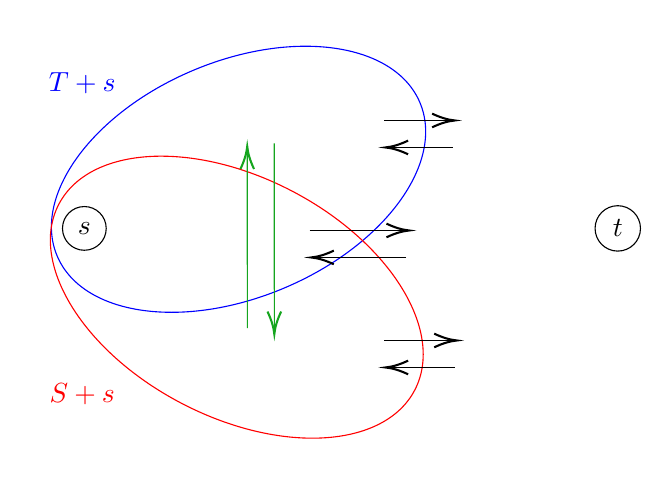
\begin{tikzpicture}[x=0.75pt,y=0.75pt,yscale=-1,xscale=1]
            %uncomment if require: \path (0,541); %set diagram left start at 0, and has height of 541

            %Shape: Ellipse [id:dp08510069255163422] 
            \draw  [color=blue] (102.91,363.31) .. controls (90.67,334.4) and (119.87,294.4) .. (168.13,273.98) .. controls (216.38,253.56) and (265.42,260.44) .. (277.66,289.35) .. controls (289.89,318.26) and (260.69,358.25) .. (212.44,378.67) .. controls (164.18,399.1) and (115.14,392.22) .. (102.91,363.31) -- cycle ;
            %Shape: Ellipse [id:dp4447445025098904] 
            \draw  [color=red] (103.7,338.37) .. controls (118.43,310.15) and (168.76,307.31) .. (216.12,332.04) .. controls (263.47,356.76) and (289.91,399.68) .. (275.18,427.9) .. controls (260.44,456.12) and (210.11,458.96) .. (162.76,434.23) .. controls (115.4,409.51) and (88.96,366.59) .. (103.7,338.37) -- cycle ;
            %Straight Lines [id:da2881669374641228] 
            \draw    (260.5,298) -- (292.5,298) ;
            \draw [shift={(294.5,298)}, rotate = 180] [color={rgb, 255:red, 0; green, 0; blue, 0 }  ][line width=0.75]    (10.93,-3.29) .. controls (6.95,-1.4) and (3.31,-0.3) .. (0,0) .. controls (3.31,0.3) and (6.95,1.4) .. (10.93,3.29)   ;
            %Straight Lines [id:da05937720730168328] 
            \draw    (293.42,311) -- (263.04,311) ;
            \draw [shift={(261.04,311)}, rotate = 360] [color={rgb, 255:red, 0; green, 0; blue, 0 }  ][line width=0.75]    (10.93,-3.29) .. controls (6.95,-1.4) and (3.31,-0.3) .. (0,0) .. controls (3.31,0.3) and (6.95,1.4) .. (10.93,3.29)   ;
            %Straight Lines [id:da610319147509233] 
            \draw    (260.5,404) -- (293.5,404) ;
            \draw [shift={(295.5,404)}, rotate = 180] [color={rgb, 255:red, 0; green, 0; blue, 0 }  ][line width=0.75]    (10.93,-3.29) .. controls (6.95,-1.4) and (3.31,-0.3) .. (0,0) .. controls (3.31,0.3) and (6.95,1.4) .. (10.93,3.29)   ;
            %Straight Lines [id:da6429005378485685] 
            \draw    (294.39,417) -- (263.06,417) ;
            \draw [shift={(261.06,417)}, rotate = 360] [color={rgb, 255:red, 0; green, 0; blue, 0 }  ][line width=0.75]    (10.93,-3.29) .. controls (6.95,-1.4) and (3.31,-0.3) .. (0,0) .. controls (3.31,0.3) and (6.95,1.4) .. (10.93,3.29)   ;
            %Straight Lines [id:da6468361291209292] 
            \draw    (224.5,351) -- (270.5,351) ;
            \draw [shift={(272.5,351)}, rotate = 180] [color={rgb, 255:red, 0; green, 0; blue, 0 }  ][line width=0.75]    (10.93,-3.29) .. controls (6.95,-1.4) and (3.31,-0.3) .. (0,0) .. controls (3.31,0.3) and (6.95,1.4) .. (10.93,3.29)   ;
            %Straight Lines [id:da5855145995489603] 
            \draw    (270.98,364) -- (227.26,364) ;
            \draw [shift={(225.26,364)}, rotate = 360] [color={rgb, 255:red, 0; green, 0; blue, 0 }  ][line width=0.75]    (10.93,-3.29) .. controls (6.95,-1.4) and (3.31,-0.3) .. (0,0) .. controls (3.31,0.3) and (6.95,1.4) .. (10.93,3.29)   ;
            %Straight Lines [id:da2652579304880732] 
            \draw [color={rgb, 255:red, 21; green, 165; blue, 30 }]   (207.47,309) -- (207.53,398.99) ;
            \draw [shift={(207.53,400.99)}, rotate = 269.97] [color={rgb, 255:red, 21; green, 165; blue, 30 }  ,draw opacity=1 ][line width=0.75]    (10.93,-3.29) .. controls (6.95,-1.4) and (3.31,-0.3) .. (0,0) .. controls (3.31,0.3) and (6.95,1.4) .. (10.93,3.29)   ;
            %Straight Lines [id:da8107260558687496] 
            \draw [color={rgb, 255:red, 21; green, 165; blue, 30 }]   (194.53,398.09) -- (194.47,312.48) ;
            \draw [shift={(194.47,310.48)}, rotate = 89.97] [color={rgb, 255:red, 21; green, 165; blue, 30 }  ,draw opacity=1 ][line width=0.75]    (10.93,-3.29) .. controls (6.95,-1.4) and (3.31,-0.3) .. (0,0) .. controls (3.31,0.3) and (6.95,1.4) .. (10.93,3.29)   ;

            % Text Node
            % \draw    (123.5, 351) circle [x radius= 14.15, y radius= 14.15]   ;
            \node[circle, draw] at (116,350) {$s$};
            % \draw (116,339) node {$s$};
            % Text Node
            \node[circle, draw] at (373,350)  {$t$};
            % Text Node
            \draw (115,430) node [color=red ] {$ S+s$};
            % Text Node
            \draw (115,280) node [color=blue] {$ T+s$};


        \end{tikzpicture}
    \end{minipage}

\end{proof}
Let's compare Greedy vs. Monotonicity.
If $r$ is monotone, then $x_{e_i}=r(S_i)-r(S_{i-1}) \geq 0$.
But if we don't care for $x \geq 0$, then we can apply Greedy.
\begin{align*}
    x\ \text{free} \implies \sum_{S:e \in S}y_S = w_e
\end{align*}
Notice that "$=$" was "$\geq$", but our previous proof showed that we
get equality anyway for the dual constraint.
\begin{conclusion}
    Greedy works for polymatroids, matroids, and general submodular functions, even with negative values.
\end{conclusion}
\begin{remark}
    Submodular $\LP$s are \emph{not} totally unimodular.
    Consider e.g. following submatrix of a submodular $\LP$:
    \[
        \det \begin{pNiceMatrix}[first-row, first-col]
                   & e_1 & e_2 & e_3 & \\
            e_1e_2 & 1   & 1   & 0     \\
            e_1e_3 & 1   & 0   & 1     \\
            e_2e_3 & 0   & 1   & 1
        \end{pNiceMatrix} = -2
    \]
    Still, we get only integer solutions, meaning submodular RHS's are special
\end{remark}
\begin{definition}
    We call a polyhedron \vocab{integral} if $P=P_I$, with $P_I$ being the
    integer hull of $P$.
    Equivalently, all vertices of $P$ are integral.
\end{definition}
We first want to derive a tool to prove that $P = P_I$.
\begin{theorem} \label{thm:lp_is_integral}
    If for all $c$ such that an optimum exist holds that
    \begin{align*}
        z \coloneqq \max \{c^Tx \mid x \in P\} \in \integers,
    \end{align*}
    then $P$ is integral.
\end{theorem}
\begin{proof}
    Let $v$ be any vertex of $P$. We know there is an outer cone of possible vectors $c$ such that $z_c = c^Tv \in \integers$.
    For $c$ long enough, we can add unit vectors and still stay in the cone,
    i.e. for any index $i$ also $z_{c_i}=(c+e_i)^Tv \in \integers$.
    Therefore, $(c+e_i)^Tv-c^Tv=v_i\in \integers$, and in particular $v \in \integers^n$
\end{proof}
In order to apply this result following definition is useful:
\begin{definition}
    We call a system $Ax \leq b$ \vocab{totally dual integral} if for all $c \in \integers^n$ with an optimum to $\{c^Tx \mid x \in P\}$
    the corresponding $y^*$ is integral.
\end{definition}
\begin{corollary}
    If $Ax \leq b$ is totally dual integral, and $b \in \integers^m$, then $P$ is integral.
\end{corollary}
\begin{proof}
    Recall that our $z$ is also the optimal objective value of the dual.
    We know for all $c$ with an optimum, that $y^* \in \integers^m$ for $b^Ty^* = z \in \integers$.
    By \autoref{thm:lp_is_integral}, all primary vertices are integral.
\end{proof}
\begin{theorem}
    For submodular $r$, the polyhedron $\{x \mid x(S) \leq r(S)\}$ is totally dual integral.
\end{theorem}
\begin{proof}
    Greedy says (note $w$ is synonym to $c$):
    \begin{align*}
        y_S^* = \begin{cases}
                    w_i - w_{i+1}, & \text{if } S=S_i, \\
                    0,             & \text{else}
                \end{cases} \in \integers^{2^E}
    \end{align*}
\end{proof}
\begin{conclusion} Note the difference:

    "Totally unimodular" corresponds to integral polyhedra for \emph{all} integer-RHS.

    "Totally dual integral" corresponds to integral polyhedra for \emph{special} RHS.
    Submodular RHS are an example.
\end{conclusion}
Consider again intersections of matroids, i.e. bipartite matchings as in \autoref{rmk:intersection_matroid}.
\begin{theorem}
    For submodular $r_1,r_2$, given the primal $\LP$
    \begin{maxi*}{x}{w^Tx}{}{}
        \addConstraint{x(S)}{\leq r_1(S)}
        \addConstraint{x(S)}{\leq r_2(S)}
        \addConstraint{x}{\geq 0}
    \end{maxi*}
    with its dual
    \begin{mini*}{y^1,y^2}{r_1^Ty^1+r_2^Ty^2}{}{}
        \addConstraint{\sum_{S:e \in S}y_S^1+y_S^2}{\geq w_e}
        \addConstraint{y^1,y^2}{\geq 0}.
    \end{mini*}
    Then the primal is totally dual integral.
\end{theorem}
\begin{proof}
    Analoguous to the proof of \autoref{thm:integer-mst-submod} we
    can show there exist optimal $(y^1)^*, (y^2)^*$ whose tight sets are nested.
    Then, we can construct following basis:
    \[
        \begin{pNiceArray}{ccrc|ccccc}[first-row, first-col]
            & S^{1,1} & \Cdots &       & S^{1,k-1} \ S^{1,k} & S^{2,l} & S^{2,l-1} & \Cdots &        & S^{2,1} \\
            e_1    & 0       & \Cdots & 0         &0 \quad  1       & 1       & 0       & \Cdots &        & 0       \\
            e_2    & 0       & \Cdots & 0 \ & 1 \quad 1       & 1       & 1       & 0      & \Cdots & 0       \\
            \Vdots &         &        &           &  \Vdots       & \Vdots        &         &        &       &         \\
            e_m    & 1       & \Cdots &           & 1 \quad 1       & 1       & \Cdots  &        &        & 1       \\
            \CodeAfter
            \line{2-4}{4-1}
            \line{2-6}{4-9}
        \end{pNiceArray}
    \]
    Notice we obtained continuous-one property, and thus totally unimodularity.
    Therefore, $y^* \in \integers^m$ as the solution to the induced linear system,
    resulting for the primal in totally dual integrality by definition.
\end{proof}
We remind ourselves of the duality of complexity and integrality:
It remains to develop an efficient optimization algorithm.
We restrict us to a cardinality (i.e. $c = \mathbf{1}$) matroid intersection algorithm:
\begin{theorem}
    For two matroids $\mathcal I_1, \mathcal I_2$, we can solve
    \begin{align*}
        \max_{I \in \mathcal I_1 \cap \mathcal I_2}|I|
    \end{align*}
    efficiently.
\end{theorem}
\begin{observe}
    A (naive) greedy approach to bipartite matchings doesn't work:
    \\
    \\
    \begin{minipage}{\textwidth}
        \centering
        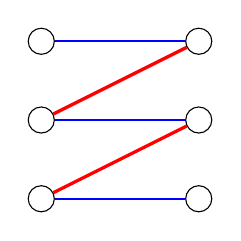
\begin{tikzpicture}
            \begin{scope}[
                    every node/.style={circle, draw},
                    every edge/.style={draw, semithick}
                ]

                \node (l1) at (0,0) {};
                \node (l2) at (0,1) {};
                \node (l3) at (0,2) {};
                \node (r1) at (2,0) {};
                \node (r2) at (2,1) {};
                \node (r3) at (2,2) {};

                \draw[red, very thick] (l1) -- (r2);
                \draw[red, very thick] (l2) -- (r3);
                \draw[blue] (l1) edge (r1);
                \draw[blue] (l2) edge (r2);
                \draw[blue] (l3) edge (r3);
            \end{scope}
        \end{tikzpicture}
        % \captionof{figure}{A graph with the spanning tree in black and arc subset $S$ in orange}
    \end{minipage}
    \vspace{5pt}
    \\
    The \textcolor{red}{red edges} form a maximum matching which isn't maximal like the \textcolor{blue}{blue set of edges}.
\end{observe}
\begin{idea}
    In order to solve the issue of wrong greedy choices we want to imitate
    an augmenting path algorithm on a bipartite graph defined by the current maximal solution $I$ and $I^c$ as partition
    and some edges connecting $I$ and $I^c$.
\end{idea}
We want to use following definition to describe the edges of our matroid-intersection-graph:
\begin{definition}[Circuit]
    A \vocab{circuit} $C$ is a minimal dependent subset in a matroid.
\end{definition}
Note that we can visualize a matroid $\mathcal I$ as a graph such that every acyclic subset is element of $\mathcal I$.
A circuit is therefore always a cycle.
\begin{example}
    The matroid over $E = \{1,2,3,4,5\}$,
    \begin{align*}
        \mathcal I = \{ &
        \emptyset,\{1\},\{2\},\{3\},\{4\},\{5\},                                                           \\
                        & \{1,2\},\{1,3\},\{1,4\},\{1,5\},\{2,3\},\{2,4\},\{2,5\},\{3,4\},\{3,5\},\{4,5\}, \\
                        & \{1,2,4\},\{1,2,5\},\{1,3,4\},\{1,3,5\},
        \{2,3,4\},\{2,3,5\},\{2,4,5\},\{3,4,5\},                                                           \\
                        & \{1,2,4,5\},\{1,3,4,5\}
        \},
    \end{align*}
    can be visualized as
    \\
    \begin{minipage}{\textwidth}
        \centering
        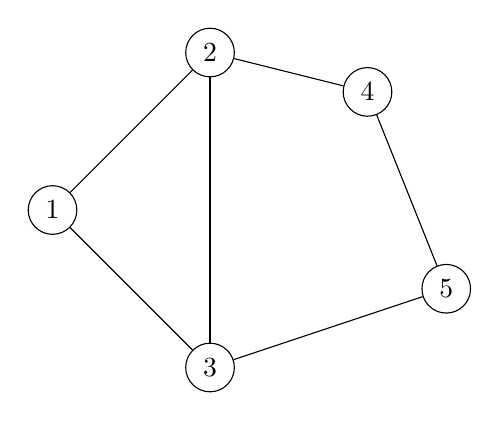
\begin{tikzpicture}
            \begin{scope}[every node/.style={circle, draw}]

                \node (1) at (0,2) {$1$};
                \node (2) at (2,4) {$2$};
                \node (3) at (2,0) {$3$};
                \node (4) at (4,3.5) {$4$};
                \node (5) at (5,1) {$5$};

                \path (1) edge (2);
                \path (3) edge (2);
                \path (3) edge (1);
                \path (2) edge (4);
                \path (3) edge (5);
                \path (4) edge (5);
            \end{scope}
        \end{tikzpicture}
    \end{minipage}
    The circuits are given as $\{1,2,3\}$, $\{2,3,4,5\}$ and $\{1,2,3,4,5\}$.
\end{example}
\begin{lemma}
    If $I \in \mathcal{I}$, but $I +e \not \in \mathcal{I}$, then $I+e$ has a unique circuit.
\end{lemma}
\begin{proof}
    We prove by contradiction. Suppose $I+e$ contains two distinct circuits $C_1,C_2$.
    Suppose w.l.o.g. that $|I|$ is minimal and $I + e = C_1 \cup C_2$.
    Then there must exist $a \in C_1 \setminus C_2$ and $b \in C_2 \setminus C_1$.

    To construct our contradiction, it suffices to show now that
    \begin{align*}
        I^\prime \coloneqq (C_1 \cup C_2)\setminus \{a,b\} \in \mathcal I.
    \end{align*}
    Suppose this doesn't hold. Then there exist a circuit $C \subset \mathcal I^\prime$.
    Then $(I - a) + e$ contains $C_2$ (since $a \not \in C_2$) and $C$
    (since $I^\prime \subset (I-a)+e$). But $|I-a|=|I|-1$ contradicts minimality of $I$.
\end{proof}
This lemma motivates following definition:
\begin{definition}
    For every $I \in \mathcal{I}$ and $e \in E$ we define
    \begin{align*}
        C(I,e)=\begin{cases}
                   \emptyset,                     & \text{if } I + e \in \mathcal I \\
                   \text{unique circuit in } I+e, & \text{else}
               \end{cases}
    \end{align*}
    as the \vocab[circuit!fundamental]{fundamental circuit}.
\end{definition}
In particular, we want to consider fundamental circuits $C_1$ of $\mathcal I_1$ and $C_2$ of $\mathcal I_2$:
Going back to our initial idea, for any $f \in I$ and $e \in I^c$, we now draw an edge iff $f \in C_1(I,e)$ or $f \in C_2(I,e)$.
